\section{Durchführung}
\subsection{Statische Methode}
\label{sec:Durchführung}
\begin{figure}
  \centering
  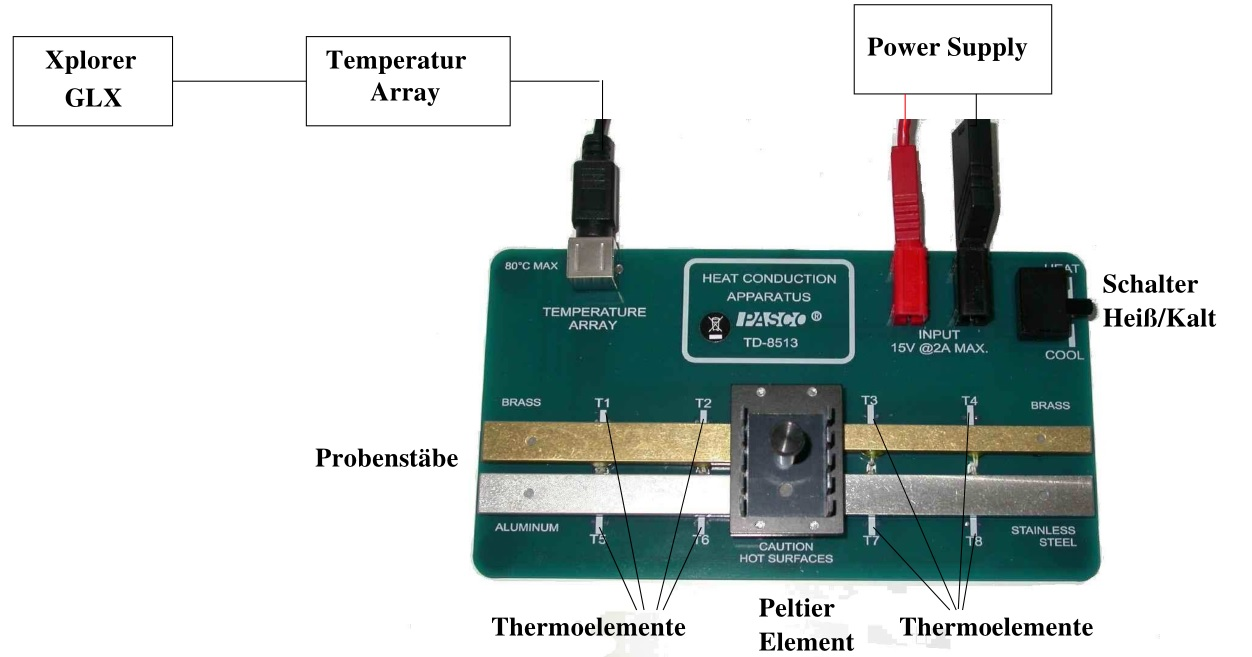
\includegraphics{data/abb1.jpg}
  \caption{Aufbau. \cite{V204}}
  \label{fig:Abb1}
\end{figure}
Es wird alles wie im Aufbau zu sehen verbunden.
Die Abtastrate wird auf 5 s gesetzt.
Am Netzgerät wird die Spannung auf 5 V geregelt, bei maximaler Stromstärke.
Auf die Metalle wird die Isolierung gelegt und der Schalter auf "HEAT" gestellt.
Nach 30 Minuten wird der Schalter wieder in die neutrale Stellung gebracht und die Aufgezeichneten Werte werden exportiert.
Dann wird die Isolierung abgenommen und zur Kühlung der Metalle der Schalter auf "COOL" gestellt, bis die Stäbe wieder eine Temperatur von unter $\SI{3}{\celsius}$ besitzen.

\subsection{Dynamische Methode}
Es wird die Abtastrate auf 2 s gesetzt.
Die Spannung am Netzgerät wird auf 8 V, bei maximaler Stromstärke eingestellt.
Die Isolierungen werden angebracht und die Messung wird gestartet.
Dazu werden die Stäbe periodisch mit einer Periode von 80 s geheizt.
Erst werden sie 40 s lang geheizt, dann 40 s lang gekühlt.
Diesen Vorgang wiederholt man für 10 Perioden.
Danach werden die Daten exportiert und die Stäbe wieder auf unter $\SI{3}{\celsius}$ gekühlt.
Dieser Vorgang wird nun mit einer Periode von 200 s wiederholt, erneut für 10 Perioden.
Anschließend werden die Werte wieder exportiert.